\section{Problem Statement}

Before stating our research problems in detail, it seems to us necessary to expose in a few paragraphs our vision of the broad context and ecosystem in which this thesis takes place.

Since the invention of the computer and later on with the Internet, many human activities have been transferred into the digital world, or said differently, virtualized or cyberized~\cite{ma2015cybermatics}. Listening to music, reading a book or the news are now mostly digital activities. Social media have pushed this trend further by virtualizing every social link humans can have: friendly relationships with Facebook, professional links with LinkedIn, photos or multimedia content sharing with EyeEm, Instagram or Tumblr, to cite a very few. Computer gaming is now the principal leisure activity at nearly all ages and is now referred to as e-sport. Large-scale virtual worlds have been created and a new culture coming from e-sport has emerged, linking together people from all around the world as this culture is completely international and does not belong to any part of the world. For example, Leagues of Legends or Clash of Clans are two different games and universes with their own rules and a really international community. The next revolution will certainly be the democratization of virtual reality, augmented reality and mixed reality. Many companies have already marketed products in these emerging fields (e.g., Oculus VR with the Oculus Rift, Microsoft with HoloLens, Samsung, Magic Leap, etc.). This evolution could made us think that our lives will become virtual in great part.

Another trend exists. The cyber world is indeed getting into the physical one by embedding computation, communication and sensing capabilities into day-to-day products with the Internet of Things (IoT). Smart things that are nowadays deeply embedded in our daily life, are not only able to sense and react to their environment but also to interact with people and things, providing valuable services to human beings. The goal of the IoT is to \say{allow people and things to be connected anytime, anyplace, with anything and anyone, ideally using any path/network and any service}~\cite{vermesan2013internet}. The IoT involves human-to-machine, machine-to-machine and human-to-human communications. Most popular IoT applications include smart homes, smart cities, smart environment, eHealth, smart supply chain, etc. For instance, smart homes propose a wide variety of domotic-related services (e.g., temperature management, user-friendly voice assistant, intrusion detection, etc.). Smart cities and smart highways monitor the traffic in real time to optimize the driving experience (e.g., diversions according to traffic jams or climatic conditions). eHealth enables patients surveillance, fall detection of elderly people, etc. Smart behavior and cooperation among many interconnected smart devices rise significant algorithmic challenges. Smart objects are not only interconnected through the Internet but may also communicate together in an ad-hoc fashion, potentially forming large-scale infrastructure-less distributed systems.
 
Among these smart objects, robotic things go one step further by providing physical services as they can act over the physical world thanks to actuation capabilities. Intelligent and networked robotic devices form the Internet of Robotic Things (IoRT)~\cite{vermesan2017internet}. Autonomous cars, collaborative floor-cleaning robots, co-working robots, etc. fall into the IoRT. Technological advances, especially in the miniaturization of robotic devices, foreshadow the emergence of large-scale ensembles of small-size robots that distributively cooperate to achieve complex tasks (e.g., modular robotic systems~\cite{yim2009modular}, swarm robotic systems~\cite{csahin2004swarm}, \gls{dimems}~\cite{bourgeois2012distributed}, etc.). These ensembles are formed from independent, intelligent and communicating units which act as a whole ensemble. These units cooperatively self-organize in order to perform specific complex tasks and achieve common goals. These systems are thought to be more versatile and more robust than conventional robotic systems while having at the same time a lower cost. When considered as a whole ensemble, a set of such units is a full IoRT object that takes part in the IoT ecosystem. At the same time, when viewed as a set of interconnected units, the ensemble is a complex intranet of robotic things, in which every unit is an embedded system with its own but limited capabilities.

In line with that trend, this dissertation deals with distributed coordination in large-scale distributed embedded systems and more specifically in resource-constrained modular robotic ensembles. The Smart Blocks~\cite{piranda2013new} and the Claytronics~\cite{goldstein-waci04} projects envision interesting applications based on large-scale modular robotic systems. The former aims to build a large distributed modular system to convey small and fragile objects, by attaching many modules together, each one equipped with a conveyance surface. The conveyance system can rearrange its global shape to self-adapt to new situations (e.g., new tasks, self-healing after a module failure, etc.). The goal of the Claytronics project is to use up to millions of micro modules to build \gls{pm}, i.e., matter that can change its physical properties in response to external and programmed events.

\gls{pm} is a physical instance of a virtual representation. This synthetic reality has a wide range of applications (e.g., sending/downloading copies of physical objects, morpheable objects reshapable at will, injectable surgical instruments, 3D interactive life-size TV, etc.). In addition, \gls{pm} could also provide a bidirectional mapping between the virtual representation of an object and its physical one formed from \gls{pm}. \gls{pm} will, therefore, be a technology which will literally bridge the gap between the physical and the virtual worlds. It will enable people not only to control their environment but also to shape it. It goes even further as it will allow them to create intelligent objects that act like living things. Implications may drastically change our society. This concept definitely fits the ultimate desire of human beings to master their world.

Modular robotics is a cross-disciplinary domain which poses both hardware and software challenges. In this thesis, we focus on software and algorithmic problems. With \gls{pm}, people will, for instance, hold in their hands large-scale networks of resource-constrained micro robotic devices. Coordination of such large-scale distributed embedded systems poses significant algorithmic issues and opens new opportunities in distributed algorithms.

In my thesis, I defend the idea that distributed high-level algorithmic primitives suitable for the coordination of these ensembles should be both identified and designed. Besides, these needs were stated during the 2016 Dagstuhl Seminar on \say{Algorithmic Foundations of Programmable Matter}~\cite{fekete2016algorithmic}. This point of view has also been recently defended by Z. Derakhshandeh in her doctoral thesis entitled \say{Algorithmic Foundations of Self-Organizing Programmable Matter}~\cite{derakhshandeh2017algorithmic}, in which she addresses the leader election, shape formation and coating problems in the theoretical Amoebot model~\cite{derakhshandeh2014brief}.

The complexity that lies in the coordination of these ensembles depends on the hardware features of the individual modules (computation power, communication model, structure organization, motion capabilities, etc.). Communication is central to module coordination. The communication model and the structure organization determine the overall network properties. Complexities of distributed algorithms are generally expressed as a function of network properties (e.g., number of nodes, number of links, node degree, radius/diameter of the system). Many algorithms target a specific class of networks. For instance, some algorithms are more efficient in sparse networks than in dense networks (e.g, the virtual coordinate-based routing protocol in~\cite{zhao2007hop}). Thus, it is crucial to take into account the network properties in order to design and choose appropriate algorithms, especially in large-scale systems.

In this work, we focus on a specific class of modular robotic systems, namely distributed modular robotic ensembles composed of resource-constrained identical modules that are organized in a lattice structure and which can only communicate with neighboring modules. We name this class of robots \acrshort{lmrs}. As explained in Section~\ref{section:context:classification}, this class captures a variety of existing systems and is particularly suitable to realize large-scale ensembles. In the same chapter, we show that these ensembles form asynchronous, sparse, low-degree, large-diameter and large-average-hop-distance networks.

The contributions of this thesis are motivated by the application scenario depicted in Figure~\ref{fig:base-application}. This scenario considers a \gls{msr}~\cite{yim2007modular} composed of more than ten thousand millimeter-scale cylindrical rolling robots developed in the Claytronics project~\cite{karagozler-iros09}. These robots move in 2D space and thus form 2D ensembles only. We call these robots the 2D Catoms, even if they are 3D objects. The term \say{catom} stands for \say{Claytronics atom}, which is the basic unit for Claytronics \gls{pm}. In our scenario, the modular robot first self-reconfigures its shape into a car shape. Then, modules into the turn-signal area coordinate themselves in order to blink in a synchronized fashion. This scenario rises several challenges. We identified and addressed three of them, namely centrality-based leader election, time synchronization and self-reconfiguration.

\begin{figure}[!h]
	\centering
	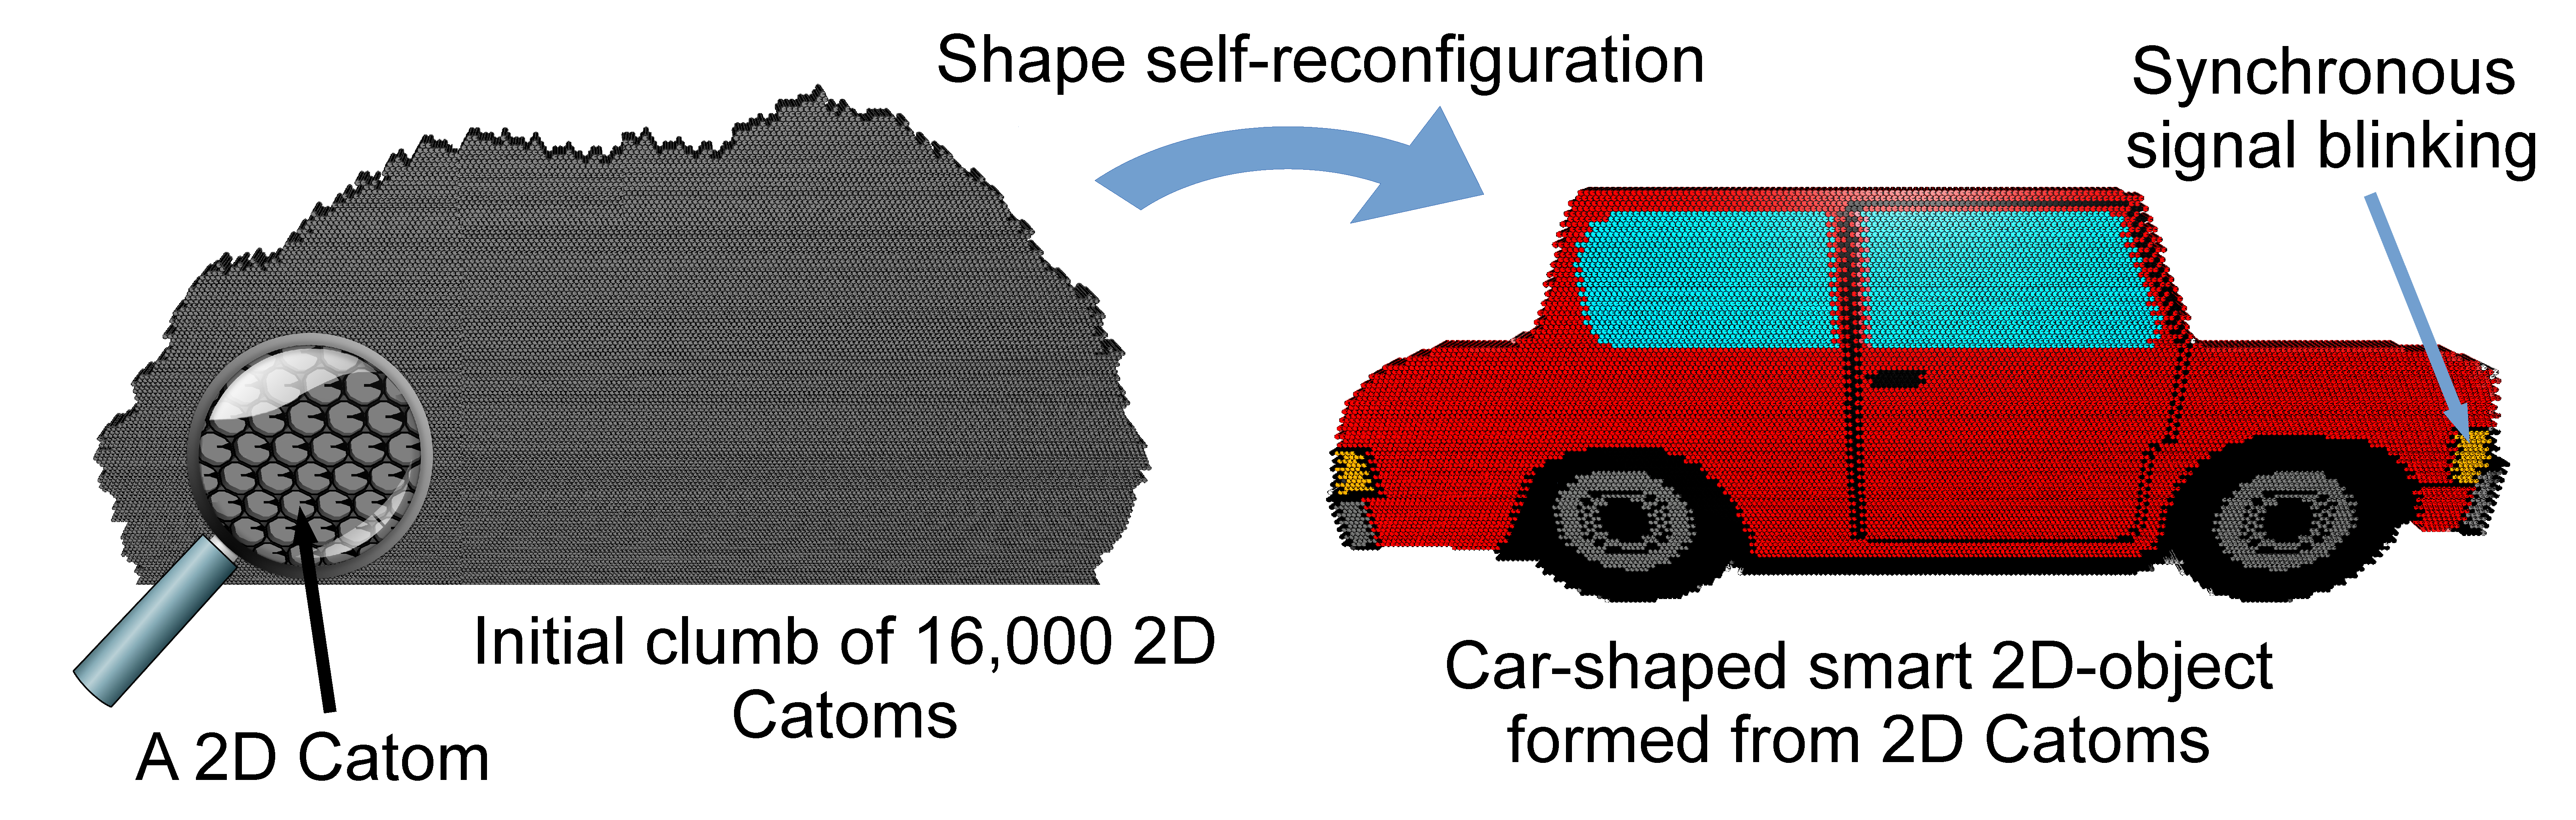
\includegraphics[width=\linewidth]{images/introduction/base-application}
	\caption{Application scenario that drives the research presented in this dissertation.\protect\footnotemark\label{fig:base-application}}
	%Illustration from http://www.fotomelia.com
\end{figure}

\footnotetext{The magnifying glass image is a modified version of an image taken from Pixabay~\url{https://pixabay.com}. To generate the 2D-Catom car image, we used a modified version of a car image taken from Fotomelia~\url{http://www.fotomelia.com}. Those two original images have been dedicated to the public domain under the Creative Commons CC0 license.}

The three algorithmic challenges we tackle in this thesis are:

\begin{description}
	\item[Self-reconfiguration] Self-reconfiguration is the process during which an \gls{msr} transforms itself from an initial configuration into a goal one. This process has several applications. In the context of programmable matter, it enables an \gls{msr} to assume different shapes. Self-reconfiguration can also be used to adapt an \gls{msr} to changes in the environment or to specific tasks. For instance, in~\cite{lakhlef2013distributed}, the authors use self-reconfiguration to rearrange the modules connectivity in order to reach an optimal network topology. Self-reconfiguration poses several software challenges. Firstly, planning is challenging as the number of possible unique configurations is huge: $(c \times w)^n$ where $n$ is the number of modules, $c$ the number of possible connections per module and $w$ the ways of connecting the modules together~\cite{yimReconf}. Depending on the physical constraints, modules can often move concurrently, which makes the configuration space grow at the rate of $O(m^n)$ with $m$ the number of possible movements and $n$ the number of modules free to move~\cite{latombe91}. The exploration space for reconfiguration between two random configurations is therefore exponential in the number of modules, which prevents us from finding a complete optimal planning for all but the simplest configurations. The optimal self-reconfiguration planning for chain-type \gls{msr}s is then an NP-complete problem~\cite{Hou2014}, and, to the best of our knowledge, nothing has been proved so far for lattice-based \gls{msr}s. Secondly, in addition to the path planning problem, the self-reconfiguration process is also challenging as it is a distributed process that requires the distributed coordination of mobile autonomous modules connected in time-varying ways. In particular, modules have to coordinate their motions in order not to collide with each other. Self-reconfiguration algorithms are often tailored for a specific class of modular robots, with specific motion constraints. Here, we base our model on the 2D Catoms. Our research question in this perspective is: How to self-reconfigure an \gls{msr} composed of thousands of 2D Catoms into various shapes?
		
	\item[Time Synchronization] Coordination (e.g., synchronous blinking) among a group of modules often relies on the existence of a common notion of time. Every module has its own notion of time provided by its own hardware clock. Since common hardware clocks are imperfect, local clocks tend to run at slightly different and variable frequencies, drifting apart from each other over time. Consequently, a distributed time synchronization is necessary to keep the local clock of each module synchronized. Several approaches to time synchronization exist (continuous vs on-demand, network-wide vs clustering, timescale transformation vs clock synchronization, etc.)~\cite{romer2005time}. The approach to be used depends on the target application. In the continuous model, nodes strive to kept synchronized at all times. This model is opposed to the on-demand synchronization model where nodes can either a posteriori agree on the time at which an event has occurred or anticipate synchronizations in order to trigger some coordinated actions at a given time. In our application scenario, we aim at simultaneously and repeatedly executing a local algorithm, namely a color change. For this specific scenario, the existence of a common notion of time among all modules is required. Here, our goal is to achieve network-wide and continuous time synchronization. This is the most general approach. Synchronization protocols based on this approach aim to keep a small offset between local clocks and a global reference time. In most of the existing protocols, devices exchange timestamped messages in order to estimate the current global time. Since time keeps going during communications, modules have to correctly compensate for network delays in order to evaluate the current global time upon reception of synchronization messages. Although it is non-trivial to accurately estimate communication delays, especially in the presence of unpredictable delays (due for example, to queueing or retransmissions), it is crucial in order to achieve high-precision performance. In this work, we assume that every module is equipped with a local clock, which can be low-precision and low-resolution, typically in the order of the millisecond. Moreover, we target fairly static ensembles. Our research on this topic is driven by the questions: How to efficiently and accurately synchronize fairly-static large-scale distributed embedded ensembles in which entities are equipped with low-precision clocks and communicate with their immediate neighbors only? What is the largest network we can synchronize and how accurately?
	
	\item [Centrality-based leader election] Many distributed algorithms require a specific role to be played by a leader, a single node in the system. The choice of this node often has a direct impact on the performance. Leaders are often used to provide such varied services as time synchronization, message routing~\cite{blazevic2005location}, etc. In many algorithms and protocols, ensuring the proper selection of the leader is crucial for the performance. In particular, selecting a central node as the leader can significantly improve algorithm efficiency by reducing the network traffic or the time of convergence, especially in large-average-distance and large-diameter networks. For example, in time-master-based synchronization protocols, placing the time-master at a central node leads to more synchronization precision in large-diameter networks as the precision of remote clock readings tends to decrease with the hop distance (see Chapter~\ref{chapter:time-synchronization}). It is thus essential to have a fast and efficient way to select a good leader. Several centrality definitions have been proposed in the literature. In this dissertation, we focus on the center and the centroid, i.e., the sets of nodes which respectively minimize the maximum and the average network distance to all the others. Classical distributed algorithms require global information about the connectivity network to elect a node that belongs to the exact center or centroid. Thus, they are not suitable for large-scale distributed embedded systems with scarce computation, memory and energy resources. Electing a central node actually involves a trade-off between the cost that can be afforded in terms of resources (time, memory, computation, energy) and the desired level of accuracy. This leads to the following research question: How to elect accurate approximate center and centroid nodes with both a reasonable convergence time and a limited memory usage in large-scale resource-constrained distributed embedded systems? 
\end{description}

It must be well understood that we use the scenario presented in Figure~\ref{fig:base-application} for illustrative purposes only. The primitives proposed in this thesis can be used to realize our scenario but we do not claim this is the only or the optimal way to do it. Moreover, this work is applicable to other applications and systems.

Although some functionalities of the 2D Catom have been physically validated by the realization of a hardware prototype (i.e., powering, adhesion and motion on a conductive surface)~\cite{karagozler-iros09}, no 2D-Catom ensemble has been erected yet and the current prototype still needs to be enhanced with different capabilities (e.g., communication). Hence, we use simulations in order to evaluate our algorithms on this platform. However, we consider that hardware deployment is an important step in the evaluation process of distributed algorithms. For experiments on hardware, we have at our disposal several dozen hardware Blinky Blocks~\cite{Kirby-chi11}. Blinky Blocks are centimeter-size modular robotic systems that were also developed in the Claytronics project. We evaluate compatible algorithms on this platform using both hardware experiments and simulations. Simulations enable evaluation in larger-scale ensembles. We present these two modular robotic systems in more detail in the next chapter.

We emphasize that our research strongly intersects with the work achieved in the fields of distributed systems, computer networks, sensor networks, ad-hoc networks, etc. In particular, centrality and time synchronization have been widely studied in the literature but rarely in ad-hoc networks composed of tens of thousands of resource-constrained devices. In this thesis, we address these problems from an efficiency and scalability perspective.

\section{Contributions}

In this thesis, we establish the network properties of our target systems and propose a collection of distributed algorithms to tackle our three research problems. It must be well understood that beyond proposing tailored contributions, our work is applicable to a variety of systems. We leverage the complete source code of all our algorithms on GitHub\footnote{GitHub repository that hosts our algorithm codes for simulations: \VisibleSimUrl{}}\footnote{Official Blinky Blocks firmware repository in which some of our algorithm codes are hosted: \url{https://github.com/claytronics/oldbb}}.

The principal contributions of this thesis are:

\begin{description}
	\item [Centrality-based leader-election algorithms] We propose a collection of efficient and effective distributed algorithms to elect approximate-centroid and approximate-center nodes in asynchronous distributed systems. We introduce the $k$-BFS SumSweep framework, the ABC-Center algorithm and the Probabilistic-Counter-based Central-Leader Election (PC2LE) framework. Frameworks are declined in two versions, one for approximate-center node election, another for approximate-centroid node election.
	Our algorithms and frameworks do not require any prior knowledge of the network, have a well-defined termination criterion, converge in a reasonable amount of time and are memory-efficient. $k$-BFS SumSweep and ABC-Center perform distributed Breadth-First Search network traversals (BFSes) from a sample of nodes, while PC2LE uses probabilistic counting:
	\begin{description}
		\item[$k$-BFS SumSweep] In the $k$-BFS SumSweep, nodes compute their partial centrality value to a subset of root nodes composed of a random initial node and $k-1$ most external nodes. Root nodes are consecutively selected using the SumSweep approach that was originally proposed as a starting point of the sequential algorithms for exact radius and diameter computation of external graphs in~\cite{borassi2014solvability}. The main idea behind our framework is that central nodes are first and foremost central to the most external ones. Let $n$ be the number of nodes in the system, $m$, the number of links and $\Delta$ the maximum network degree. Our framework runs in $O(kd)$ time using $O(mn^2)$ messages of size $O(1)$ and $O(\Delta)$ memory space per node\footnote{We adopt a system approach to quantify the asymptotic memory usage of our algorithms. Unless otherwise mentioned, memory complexities are expressed in machine words rather than in bits (see Section~\ref{section:centrality:model}). The size of words, however, limits the number of nodes the network may contain. For instance, we assume that a node identifier is stored using a single word, thus, $O(1)$ memory space. If a word is composed of $w$ bits, then the network may only contain up to $2^w$ nodes.}. As shown in the evaluation section, our framework provides good accuracy with small $k$ values even in large-scale Blinky Blocks systems with more than $10^4$ modules.
		\item [ABC-Center] ABC-Center\footnote{Some examples of ABC-Center executions on Blinky Blocks systems are available online in video at \url{https://youtu.be/QxK12UAq42o} and \url{https://youtu.be/PYnJn6tXKa8}} extends the sequential Minimax~\cite{handler1973minimax} and 4-Sweep~\cite{crescenzi2013computing} algorithms. ABC-Center identifies an extreme path and recursively isolates midpoints on it until electing a single node. The main idea of ABC-Center is that central nodes lie in the middle of a diameter path. ABC-Center may be more convenient to use than the $k$-BFS framework as ABC-Center converges by itself, i.e., its termination does not rely on any input parameter. We propose two versions of ABC-Center. The latest version, ABC-CenterV2, runs in $O(sd)$ time using $O(mn^2)$ messages of size $O(1)$ and $O(\Delta)$ memory space per node, where $s$ is the number of iterations that ABC-CenterV2 requires to terminate. ABC-Center requires only a few iterations in Blinky Blocks systems where nodes are organized in a simple-cubic lattice.
		\item [Probabilistic-Counter-based Central-Leader Election (PC2LE)] PC2LE is based on the input-graph analysis algorithms~\cite{kang2011centralities,kang2011hadi} and the distributed synchronous algorithm~\cite{garin2012distributed} which use low-memory-footprint probabilistic counters (e.g., Flajolet-Martin~\cite{flajolet1985probabilistic}, HyperLogLog~\cite{flajolet2007hyperloglog}) to estimate node centrality measures. In PC2LE, an estimated centrality value is computed for all nodes. PC2LE is approximately equivalent to running a BFS from every node but at less expense in terms of computations and communications. PC2LE runs in $O(d)$ time using $O(mn^2)$ messages of size $O(c)$ and $O(\Delta + c)$ memory space per node, where $c$ is the memory complexity of the probabilistic counter that is used.
	\end{description}
	To the best of our knowledge, our algorithms are the most precise existing distributed algorithms designed to elect an approximate centroid or an approximate center in our target systems, with both a reasonable convergence time and a limited storage cost.

	\item [Modular Robot Time Synchronization Protocol (MRTP)\footnote{Some examples of MRTP running on the Blinky Blocks platform are available online in video at \url{https://youtu.be/66D12ESGc98} and \url{https://youtu.be/X6QzivsmJBo}}] We propose MRTP, a network-wide time synchronization protocol for modular robots with neighbor-to-neighbor communications. Our protocol achieves its performance by combining several mechanisms: central time-master election, selection of the most suited mechanism to compensate for communication delays depending on the target system and clock skew compensation using linear regression. MRTP is strongly inspired by time synchronization protocols proposed in ad-hoc wireless sensor networks (the Timing-sync Protocol for Sensor Networks (TPSN)~\cite{ganeriwal2003timing}, the Flooding Time Synchronization Protocol (FTSP)~\cite{maroti2004flooding} and the PulseSync protocol~\cite{lenzen2009optimal}). We evaluate our protocol on the Blinky Blocks system both on hardware and through simulations. Experimental results show that MRTP can potentially manage real systems composed of up to 27,775 Blinky Blocks. We show that our protocol is able to keep a Blinky Blocks system synchronized to a few milliseconds, using few network resources at runtime, even though the Blinky Blocks hardware clocks exhibit very poor accuracy and resolution. We compare MRTP to existing synchronization protocols ported to fit our system model. Simulation results show that MRTP exhibits on average a lower maximum pairwise synchronization error than the most precise compared protocols while sending more than half less messages in compact systems.
	\item [Cylindrical-Catoms Self-Reconfiguration (C2SR) algorithm\footnote{Some examples of self-reconfiguration with C2SR are available online in video at \url{https://youtu.be/XGnY-oS4Nw0}}] We propose C2SR, a self-reconfiguration algorithm for rolling cylindrical modules arranged in a two-dimensional vertical hexagonal lattice. Our algorithm is a parallel, asynchronous and decentralized distributed algorithm to self-reconfigure robots from an initial configuration into a goal one. It is able to manage almost any kind of initial and goal compact shapes (i.e., without any hole). Although our work is focused on the algorithm, we carry out our analysis with respect to the hardware constraints of the 2D Catoms. C2SR extends the algorithm in~\cite{rubenstein2014programmable} proposed for swarm robotic systems which assume different mechanical constraints. C2SR is a step toward realizing programmable matter. We evaluate our algorithm through simulation of large ensembles composed of more than ten thousand modules. We show the effectiveness of our algorithm and study its performance in terms of communications, movements and execution time. Our observations indicate that the number of communications, the number of movements and the execution time of our algorithm are highly predictable. Furthermore, we observe execution times that are linear in the size of the goal shape.
\end{description}

\section{Outline}

This dissertation is organized as follows. In Chapter~\ref{chapter:context}, we present the context of this thesis, including the specific features of our target modular robotic systems. Research problems are then addressed in three separate chapters. In Chapter~\ref{chapter:centrality}, we present our work on network centrality. Afterwards, we develop our work on time synchronization in Chapter~\ref{chapter:time-synchronization}. Our work on self-reconfiguration is presented in Chapter~\ref{chapter:self-reconfiguration}. These three contribution chapters are organized in a similar way. First, we briefly explain the research problem once more and then state the system model. Then, we provide a comprehensive overview of the state of the art on that problem. After that, we detail our contribution(s) and subsequently present experimental results before concluding the chapter. Finally, in Chapter~\ref{chapter:conclusion}, we summarize the contributions of this thesis and propose some directions for future work.